\chapter{Reconstruction and Selection}%
\label{ch:recon}

At the top level events are required to have one Higgs boson candidate and one
vector boson candidate. In all cases a Higgs boson candidate is comprised of two
$b$-jets. More on the jet collection and $b$-tagging strategy used in
section~\ref{sec:jets}. Vector boson candidates are characterised by a number of
different decay products defined in section~\ref{sec:lepton}, these decay
products trigger the recording of events, specific triggers used are discussed
in section~\ref{sec:triggers}. Reconstruction of basic quantities as well as
higher level algorithms such as overlap removal are handled by Athena and the
CxAOD Framework, more on these in section~\ref{sec:cxaod}. Finally with all
quantities reconstructed events are categorised in different analysis regions,
these are described in section~\ref{sec:ana-regions}.

My contributions to the reconstruction and selection include maintenance of the
CxAOD Framework, running production campaigns to produce new datasets when
impactful changes have been made further up the analysis chain, and implementing
new systematic uncertainties in the CxAOD Framework (not discussed until
chapter~\ref{ch:systematics}).

\section{Athena and the CxAOD Framework}
\label{sec:cxaod}
Data recorded by the ATLAS detector is passed through the central collaboration
software framework Athena before entering the analysis level data processing.
\begin{figure}[h]
  \centering
  %Define block styles
  \tikzstyle{decision} = [diamond, draw, fill=blue!20, 
  text width=4.5em, text badly centered, node distance=3cm, inner sep=0pt]
  \tikzstyle{block} = [rectangle, draw, fill=blue!20, text width=12em, text
  centered, rounded corners, minimum height=3em]
  \tikzstyle{line} = [draw, -latex']
  \tikzstyle{cloud} = [draw, ellipse,fill=red!20, node distance=3cm, minimum
  height=2em]
  
    
  \begin{tikzpicture}[node distance = 2cm, auto]
    % Place nodes
    \node [block] (gen) {Generation};
    
    \node[below=0.75cm of gen] (gen-half) {};
    \node[right=0.75cm of gen-half] (evnt) {EVNT};
    
    \node [block, below=1.5cm of gen] (sim) {Simulation};

    \node[below=0.75cm of sim] (sim-half) {};
    \node[right=0.75cm of sim-half] (hits) {HITS};
    
    \node [block, below=1.5cm of sim] (digi) {Digitisation};

    \node[below=0.75cm of digi] (digi-half) {};
    \node[right=0.75cm of digi-half] (rdo) {RDO};
    
    \node [block, below=1.5cm of digi] (mc-reco) {Reconstruction};

    \node[below=0.75cm of mc-reco] (mc-reco-half) {};
    \node[right=0.75cm of mc-reco-half] (xaod) {xAOD};
    
    \node [block, below=1.5cm of mc-reco] (mc-der) {Derivation};

    \node[below=0.75cm of mc-der] (mc-der-half) {};
    \node[right=0.75cm of mc-der-half] (dxaod) {DxAOD}; 
    
    \node [block, left=3cm of digi, fill=red!20] (trig) {Trigger};

    \node[below=0.75cm of trig] (trig-half) {};
    \node[left=0.75cm of trig-half] (dxaod) {RAW};
    
    \node [block, below=1.5cm of trig, fill=red!20] (data-reco) {Reconstruction};

    \node[below=0.75cm of data-reco] (data-reco-half) {};
    \node[left=0.75cm of data-reco-half] (xaod) {xAOD};
    
    \node [block, below=1.5cm of data-reco, fill=red!20] (data-der) {Derivation};

    \node[below=0.75cm of data-der] (data-der-half) {};
    \node[left=0.75cm of data-der-half] (dxaod) {DxAOD};

    \node[left=1.5cm of mc-der] (ghost) {};
    \node [block, below=1.5cm of ghost, fill=purple!40] (ana) {Analysis};
    
    % Draw edges
    \path [line] (gen) -- (sim);
    \path [line] (sim) -- (digi);o
    \path [line] (digi) -- (mc-reco);
    \path [line] (mc-reco) -- (mc-der);

    \path [line] (trig) -- (data-reco);
    \path [line] (data-reco) -- (data-der);

    \path [line] (mc-der) -- (ana);
    \path [line] (data-der) -- (ana);
  \end{tikzpicture}
  \caption{A flow chart showing the Athena data processing chain. Red nodes
    indicate the presence of data recorded from collisions and blue nodes indicate the
    presence of Monte-Carlo simulated events.}
  \label{fig:data-flow}
\end{figure}

Athena is responsible for the steps shown in figure~\ref{fig:data-flow}. As can
be seen in the figure Athena processes both data recorded from collisions and
Monte-Carlo simulated predictions. Steps up until and including reconstruction
are required to transform the raw or simulated read-out of the detector into
what are known as physics objects. These physics objects correspond to
ultra-violet and infra-red safe descriptions particles and hadron showers e.g.
leptons and jets. Given the initial transverse energy of the collisions (zero)
any missing transverse energy ($E_{\mathrm{T}}^{\text{miss}}$) is also reconstructed based
on the sum of the transverse energy of all objects in an event, this missing
energy indicates the presence of particles in the event that cannot be detected
by any of the ATLAS subsystems. The only particles in the Standard Model for
which this is expected are neutrinos. The files containing the reconstructed
physics objects adhere to the ATLAS Event Data Model and are referred to as
Analysis Object Data (xAOD). After reconstruction a part of Athena called the
derivation framework is used to produce skimmed and slimmed xAODs known as
Derived xAODs (DxAODs). The reduction of these files is carried out based on a
loose selection criteria.

DxAODs are the usual starting point for analysis level software, in the case of
this analysis the CxAOD Framework. As in in figure~\ref{fig:cxaod-flow}
\begin{figure}[ht]
  \centering
  
  \tikzstyle{decision} = [diamond, draw, fill=blue!20, 
  text width=4.5em, text badly centered, node distance=3cm, inner sep=0pt]
  \tikzstyle{block} = [rectangle, draw, fill=blue!20, text width=12em, text
  centered, rounded corners, minimum height=3em]
  \tikzstyle{line} = [draw, -latex']
  \tikzstyle{cloud} = [draw, ellipse,fill=red!20, node distance=3cm, minimum
  height=2em]
  
    
  \begin{tikzpicture}[node distance = 2cm, auto]
    % Place nodes
    \node [cloud] (xAOD) {xAOD};
    \node[cloud, left=3cm of xAOD] (DxAOD) {DxAOD};
    \node[left=1.5cm of xAOD] (ghost) {};

    \node[block, below=1.5cm of ghost] (CxAODMaker) {CxAOD Maker};
    \node[cloud, below=1.5cm of CxAODMaker] (CxAOD) {CxAOD};

    \node[block, below=1.5cm of CxAOD] (CxAODReader) {CxAOD Reader};
    \node[below=1.5cm of CxAODReader] (ghost2) {};

    \node[cloud, left=1.5cm of ghost2] (nTuple) {nTuple};
    \node[cloud, right=1.5cm of ghost2] (hist) {Histograms};

    \node[block, below=1.5cm of hist] (fit) {Fitting Framework};
    \node[block, below=1.5cm of nTuple] (rd) {Research \& Development};
    
    % Draw edges 
    \path [line] (xAOD) -- (CxAODMaker);
    \path [line] (DxAOD) -- (CxAODMaker);
    
    \path [line] (CxAODMaker) -- (CxAOD);
    \path [line] (CxAOD) -- (CxAODReader);

    \path [line] (CxAODReader) -- (nTuple);
    \path [line] (CxAODReader) -- (hist);

    \path [line] (hist) -- (fit);
    \path [line] (nTuple) -- (rd);
  \end{tikzpicture}
  \caption[Data flow of the analysis.]{A flow chart showing the CxAOD Framework
    data processing chain. The red elliptical nodes indicate data formats and
    the blue rectangular nodes indicate software modules.}
  \label{fig:cxaod-flow}
\end{figure}

The CxAOD Framework has two major modules the Maker and the Reader. The job of
the Maker is to further slim the data by performing pre-selection cuts and also
to apply calibrations which will be detailed below, the output of the Maker is
called a Calibrated xAOD (CxAOD). The Reader takes a CxAOD as input and performs
the analysis event selection, it can output histograms or $N$-tuples.

The Maker applies the selections of each of the three analysis channels, defined
in section~\ref{sec:selection}. CxAODs are produced separately for each of the
three channels as the different background compositions and signal signatures
require different optimisation. Pre-selection is performed on jets based on
requirements of transverse momentum and pseudo-rapidity. A tool known as the Jet
Vertex Tagger (JVT) is used to remove jets resulting from pileup from events.

\section{Leptons}%
\label{sec:lepton}

The channels of the \VHbb\ analysis are defined by the number of
observed charged leptons ($e$ or $\mu$) in the decay of the vector boson. There
is one channel for the study of \WHbb\ decays where the leptonic
decay $W \rightarrow \ell\nu$ yields a single charged lepton, the 1--lepton
channel. There are two channels for the study of \ZHbb\ decays, the
0--lepton channel where $Z \rightarrow \nu\nu$, and the 2--lepton channel where
$Z \rightarrow \ell\ell$.

Two classifications of lepton are defined in order to categorise events into the
individual channels of the analysis, these are called \VH-loose and \VH-signal
leptons, channels are defined as disjoint sets by requiring different numbers of
both lepton categories. These classifications are defined in
table~\ref{tab:vh-leptons}.
\begin{table}
  \centering
  \resizebox{\textwidth}{!}{%
  \begin{tabular}{ l l l l l l l}
    \toprule
    \bfseries{Name} & $\bm{p_T}$ &  $\bm{\lvert \eta \rvert}$ & \bfseries{ID} & $\bm{d_0^{sig}}$ & $\bm{\lvert \Delta z_0\sin{\theta} \rvert}$
    & \bfseries{Isolation}\\
    \midrule
    \multicolumn{7}{l}{\bfseries{electrons}}\\
    VH-loose & > 7 \\GeV  & < 2.47 & LH Loose & < 5 & < 0.5 mm & FCLoose \\
    ZH-signal & > 27 \\GeV & < 2.47 & LH Loose & < 5 & < 0.5 mm & FCLoose \\
    WH-signal & > 27 \\GeV & < 2.47 & LH Tight & < 5 & < 0.5 mm & FixedCutHighPtCaloOnly \\
    &&\\
    \multicolumn{7}{l}{\bfseries{muons}}\\
    VH-loose & > 7 \\GeV & < 2.7 & Loose quality & < 3 & < 0.5 mm & FixecdCutLoose \\
    ZH-signal & > 27 \\GeV & < 2.5 & Loose quality & < 3 & < 0.5 mm & FixecdCutLoose \\
 WH-signal & > 27 \\GeV & < 2.5 & Medium quality & < 3 & < 0.5 mm & FixedCutHighPtCaloOnly \\
    \bottomrule
  \end{tabular}
  }
  \caption{Definitions of the VH leptons used to define and select events for
    the three analysis channels where $d_0^{sig}$ is the measured with respect to
    the beam line. }
  \label{tab:vh-leptons}
\end{table}
The characteristics of the fake lepton background from QCD multi-jet processes
differs between the 1-- and 2--lepton channels hence the reason for two
different categorisations. In general to suppress this kind of background
leptons are required to be isolated from other detector activity.

\subsection{Electrons}
\label{subsec:electrons}

As mentioned in chapter~\ref{ch:detector} electrons leave tracks in the ID and
energy deposits in the ECAL. Reconstructing electrons requires clustering the
energy deposits in the ECAL, this is achieved with a sliding window
algorithm~\cite{Delmastro:1747242}. Clusters must then be associated to tracks
in the ID, a Gaussian Sum Filter~\cite{ATLAS-CONF-2012-047} is used to account
for energy loses due to bremsstrahlung radiation. The energy for electron
candidates must be calibrated before it can be used in order to account for
things such as non-uniformity in the detector response. Calibration is achieved
by using simulated cluster activity from single particles to train a BDT
regression model designed to regress the measured energy in the ECAL to the
simulated energy. An in-situ data driven correction is applied to normalise the
response between data and simulation~\cite{ATL-PHYS-PUB-2016-015}.

Reconstruction alone is not enough to find electrons, other particles may leave
similar signatures in the ATLAS sub-detectors and therefore electron
identification must also be performed. Identification is performed using a
likelihood-based method. Variables which have power to discriminate between
electrons and other particles are used in the likelihood such as shower
profiles, track quality, how closely track and cluster positions match in $\eta$
and $\phi$, and the presence of a high-threshold TRT hit. This is one of the
main benefits of the TRT. Performance of this method is well
studied~\cite{ATLAS-CONF-2016-024,EgammaEffTWiki}.

\subsection{Muons}

Finding muons in the detector requires consideration of the coverage of the
different ATLAS sub-detectors, especially as in general muons are not stopped in
the detector. Muons leave charged tracks in the ID and the muon spectrometers
which have coverages of $\lvert \eta \rvert < 2.7$ and $\lvert \eta \rvert <
2.5$ respectively. For the region $\lvert \eta \rvert > 2.5$ a stand-alone
algorithm which doesn't use ID tracks can be used. All muons within the coverage
of the ID require good quality ID tracks~\cite{muonTWiki,
  MuonSelectionToolTwiki}. A combined algorithm is used in the majority of
cases. For the region $\lvert \eta  \rvert < 0.1$ two specialised algorithms
SegmentTagged and CaloTagged are used, which require only muon segment and
calorimeter deposits respectively. All aforementioned algorithms are used
together in what is known as a unified
chain~\cite{Aad:2014rra,MuonChainTWiki,ATL-PHYS-PUB-2015-037} to reconstruct and
identify muons.

\subsection{Taus}

As mentioned the only charged leptons that are considered in the analysis are
electrons and muons, leptonically decaying taus will include these as the only
visible decay products, hadronically decaying taus must be considered
separately. Decays are considered as one or three pronged based on the number of
charged decay products, pions, with neutrinos and neutral pions also present.
These decays are reconstructed in the calorimeters like jets with the anti-$k_t$
algorithm with $\Delta R = 0.4$~\cite{ATL-PHYS-PUB-2015-045} but the $p_{\mathrm{T}}$ of
the tau is set to the total energy of the TopoClusters within $\Delta R < 0.2$,
more on TopoClusters in section~\ref{sec:jets}. Tau candidates must have $p_{\mathrm{T}} >
20 \GeV$, $\lvert  \eta \rvert < 2.5$ excluding $1.37 < \lvert \eta \rvert <
1.52$, and either exactly 1 or 3 tracks. A BDT based method for tau
identification is used to reject fakes. The number of medium quality taus is
included in each event~\cite{TauRecommendation2015,TauRecommendation2016}.

\section{Triggers}
\label{sec:triggers}

As stated at the beginning of this chapter the decay products of the vector
boson candidate are used to trigger the recording of events for this analysis.
Important triggers are the $E_{\mathrm{T}}^{\text{miss}}$, single electron and single muon
triggers. Note that it is not necessary to trigger on both charged leptons
coming from the Z boson in the 2--lepton channel, the presence of one lepton
allows the triggering to occur and the requirement of 2 leptons can be imposed
at a later stage. Some events will be missed by not using a di-lepton trigger,
however these amount to approximately only 5\% of the
total~\cite{VHObjectNote2019}. The list of triggers used as they appear in the
ATLAS trigger menu are shown in table~\ref{tab:triggers}, for the
$E_{\mathrm{T}}^{\text{miss}}$, electron and muon triggers respectively.
\begin{table}[h]
  \begin{center}
    \resizebox{0.95\textwidth}{!}{
      \begin{tabular}{ l l l p{7cm} }
        \toprule
        \textbf{ Trigger Name } & \textbf{Period} & \textbf{Threshold (GeV)} & \textbf{Description} \\
        \midrule
        \multicolumn{4}{l}{\bfseries{$\bm{E_T^{miss}}$}}\\
        HLT\_xe70\_L1XE50 & 2015 & 70 GeV & \multirow{4}{*}{\parbox{6.5cm}{Seeded using the level L1\_XE50 (L1\_XE55) LAr and Tile calorimeter triggers, calibrated at the EM scale, with a threshold of 50(55) GeV.}} \\
        HLT\_xe90\_mht\_L1XE50 & 2016 (A-D3) & 90 GeV &  \\
        HLT\_xe110\_mht\_L1XE50  & 2016 ($\geq$ D4) & 110 GeV & \\
        HLT\_xe110\_pufit\_L1XE55 & 2017 & 110 GeV &  \\
        HLT\_xe110\_pufit\_xe70\_L1XE50 & 2018 & 110 GeV & \\
                                &&&\\
        \multicolumn{4}{l}{\bfseries{electrons}}\\
        HLT\_e24\_lhmedium\_L1EM20VH & 2015 & 24 GeV & Seeded using L1EM20VH level 1 trigger calibrated at the EM scale with a threshold of 20 GeV, and require medium ID quality.\\
                                &&&\\
        HLT\_e60\_lhmedium & 2015 & 60 GeV  & Seeded using L1EM20VH level 1 trigger calibrated at the EM scale with a threshold of 20 GeV, and require medium ID quality.\\
                                &&&\\
        HLT\_e120\_lhloose & 2015 & 120 GeV & Seeded using L1EM20VH level 1 trigger calibrated at the EM scale with a threshold of 20 GeV, and require loose ID quality.\\
                                &&&\\
        HLT\_e26\_lhtight\_nod0\_ivarloose & 2016 -- 2018 & 26 GeV & Tight likelihood ID required, and variable loose isolation required\\
        HLT\_e60\_lhmedium(\_nod0) & 2016 -- 2018 & 60 GeV & Medium ID likelihood required\\
        HLT\_e140\_lhloose(\_nod0) & 2016 -- 2018 & 140 GeV & Loose ID likelihood required\\
        HLT\_e300\_etcut & 2018 & 300 GeV & No ID requirements. \\
                                &&&\\
        \multicolumn{4}{l}{\bfseries{muons}}\\
        HLT\_mu20\_iloose\_L1MU15 & 2015 & 20 GeV & Seeded using L1MU15 level 1 trigger with a threshold of 15 GeV, and requiring loose isolation requirements.\\
                                &&&\\
        HLT\_mu50\ & 2015 -- 2018 & 60 GeV  & No isolation requirements. \\
        HLT\_mu26\_ivarmedium & 2016 -- 2018 & 26 GeV & Variable cone medium isolation requirements \\
        \bottomrule
      \end{tabular}
    }
    \caption{ Triggers used during the 2015, 2016, 2017 and 2018 data collection
      periods, notation like A or D3 denote periods during the year. }
    \label{tab:triggers}
  \end{center}
\end{table}

\subsection{0--Lepton Channel Triggers}
The events in the 0--lepton channel should have a $qq\nu\nu$ final state. We use
the $E_{\mathrm{T}}^{\text{miss}}$ triggers listed in table~\ref{tab:triggers} as the final
state will manifest in the detector as $E_{\mathrm{T}}^{\text{miss}}$ with the presence of
jets. At the stage of triggering $E_{\mathrm{T}}^{\text{miss}}$ is only calculated from
energy measured in the calorimeters. As muons do not deposit much energy in the
calorimeters the $W \to \mu \nu + \text{jets}$ process is used to study the
trigger efficiency and derive an appropriate scale factor (the energy of the
muon provides constraints on the energy of the neutrino).

\subsection{1-- and 2--Lepton Channel Triggers}
The 1-- and 2--lepton channel's final states are $qq\ell\nu$ and $qq\ell\ell$
respectively. As the 2--lepton channel events are not expected to contain
significant $E_{\mathrm{T}}^{\text{miss}}$ and inefficiencies in the muon trigger are
mitigated by the requirement of two muons, the single lepton triggers listed in
table~\ref{tab:triggers} are simply used without any $E_{\mathrm{T}}^{\text{miss}}$
triggers. In the 1--lepton channel there is significant $E_{\mathrm{T}}^{\text{miss}}$
expected due to the presence of the neutrino. Single lepton triggers are used
for events with $75~\GeV < p_{\mathrm{T}}^{V} < 150 \GeV$ where the $E_{\mathrm{T}}^{\text{miss}}$
triggers have yet to turn on fully, for events with $p_{\mathrm{T}}^{V} > 150~\GeV$ in
order to mitigate inefficiencies in the single muon triggers similar
$E_{\mathrm{T}}^{\text{miss}}$ triggers to the 0--lepton triggers are used in conjunction
with the single lepton triggers.

\section{Jets}
\label{sec:jets}

As mentioned in chapter~\ref{ch:theory} jets are the roughly conical structure
of detector activity resulting from the hadronisation of a QCD parton. Two
categories of jets are considered, signal jets and forward jets, when the number
of total jets is referred to it is equal to the sum of signal and forward jets.
As the Higgs candidate in every channel of the analysis consists of two
$b$-jets, both the reconstruction of jets and the $b$-tagging strategy have huge
impacts on the final measurements. In this section the way jets are found and
reconstructed will be introduced, $b$-tagging will be explained in general and
then the specific tagging strategy of the analysis will be detailed.

\subsection{Topological Calorimeter Cluster Anti-$k_t$ Jets}
The jets that are found with a given algorithm are referred to as a jet
collection. The jet collection relevant to this analysis uses topological
calorimeter cell clusters to reconstruct jets~\cite{CALO2008}. These cluster are
then passed to the anti-$k_t$ jet finding algorithm~\cite{anti-kt}. This
algorithm takes a radius parameter which governs the size of jets, a radius
parameter of $R=0.4$ is chosen.

As mentioned in chapter~\ref{ch:detector} pileup can cause issues with
reconstruction. In general there is a desire to suppress any jets which arise
from pileup. The Jet Vertex Tagger (JVT) is a likelihood-based discriminant
which is used to achieve this. The primary vertex location, jet $p_{\mathrm{T}}$ and the
$p_{\mathrm{T}}$ of tracks associated to a given jet, serve as inputs to the JVT which
outputs a 2-D likelihood that the jet arises from pileup. The likelihood is
resilient to bias arising from the jet flavour. The tool is applied only to jets
in region $\lvert  \eta \rvert < 2.5$ and $p_{\mathrm{T}} > 120$~\GeV. A cut of JVT = 0.59,
is applied to all jets in the collection, this cut has an average efficiency of
92~\%. The definitions of signal and forward jets can be found in
table~\ref{tab:jet-cats}.
\begin{table}[h]
  \centering
  \begin{tabular}{l l}
    \toprule
    {\bfseries Jet Category} & {\bfseries Selection Requirements} \\
    \midrule
    Forward Jets & jet cleaning \\
    & $p_{\mathrm{T}} > 30\,\GeV$ \\
    & $2.5 \leq \left|\eta\right| < 4.5$ \\ 
    %\hdashline \\[1ex]
    &\\
    Signal Jets & jet cleaning \\
    & $p_{\mathrm{T}}} > 20\,\GeV$ \\
    & $ \left|\eta\right| < 2.5$ \\ 
    & JVT medium for $p_{\mathrm{T}}} < 120\,\GeV$ \\
    \bottomrule
  \end{tabular}
  \caption[Jet selection requirements.]{Details of jet selection requirements
    where jet cleaning refers to the quality criteria specified in the
    JetCleaningTool, which is included in
    Athena~\cite{ATLAS-CONF-2015-029,Gonski:2272136}.}
  \label{tab:jet-cats}
\end{table}

\subsection{\texorpdfstring{$b$}{b}-tagging}
\label{sec:btagging}

It is important to distinguish jets originating from $b$-quarks, which form our
Higgs candidate, from $c$-jets and $\tau$-jets, as well as jets originating from
quarks lighter than $c$-quark which are categorised together as light-jets. The
calculation of a discriminant which ought to separate $b$-jets from other jets is
known as $b$-tagging. In order to develop such a discriminant one must use
simulated predictions in which the flavour of the parton which initiated a given
jet is known so that the performance of the discriminant can be validated. In
simulation a jet and the parton that initiated that jet are distinctly separate
objects and so a set of rules must be defined in order to decide which jet is
$b$-jet and likewise for other types of jets. Those rules are as follows:
\begin{enumerate}
\item  If a weakly decaying $b$-hadron is found within $\Delta R<R_{\text{max}}$ of the
  jet axis, the jet is labeled a $b$-jet.
\item  If a $b$-hadron isn't found, but a weakly decaying $c$-hadron is
  found within $\Delta R<R_{\text{max}}$ of the jet axis, then the jet is labeled as a $c$-jet.
\item  Otherwise, if a $\tau$-lepton is found within
  $\Delta R<R_{\text{max}}$ of the jet axis, the jet is labeled a $\tau$-jet.
\item If any one hadron or $\tau$-lepton matches more than one jet, the closest jet
  is chosen as its parent.
\item All unlabeled jets after steps 1 through 4 are labeled as light-jets.
\end{enumerate}

The algorithm used to tag $b$-jets is the MV2c10 algorithm, this is a BDT which is
trained on kinematic and structural information about each jet. It is setup to
categorise between $b$-jets (signal) and a mixture of light-jets and $c$-jets
(background). The events in the training sample are simulated $t\bar{t}$ events
that have at least one lepton coming from a leptonically decaying $W$ boson, and
hadronically decaying $Z^\prime$ events. The training sample has 5 million
$t\bar{t}$ events and 3 million $Z^\prime$ events.

The kinematic training variables that enter into the MV2c10 algorithm are simply
the jet $p_{\mathrm{T}}$ and $\eta$. The structural information is more complicated, IP2D
and IP3D are two algorithms based on a log-likelihood ratio discriminant of
impact parameters (see chapter~\ref{ch:detector}). IP3D is defined as
\begin{align}
  \text{IP3D} &=\sum_{i=1}^{N}\log{\frac{p_b}{p_u}} \\
  \text{where}& \notag \\
  p_b &= P\Big(\text{is }b\text{-jet} \Big\vert \frac{d_0}{\sigma_{d_0}},
        \frac{z_0 \sin{\theta}}{\sigma_{z_0\sin{\theta}}}\Big),\\
  p_u &= P\Big(\text{is light-jet} \Big\vert \frac{d_0}{\sigma_{d_0}},
        \frac{z_0 \sin{\theta}}{\sigma_{z_0\sin{\theta}}}\Big),\\
  \text{and} & \notag \\
  N &= \text{the number of tracks for a given jet.} \notag
\end{align}
IP2D has the same definition but the probabilities $p_b$ and $p_u$ are
conditional only on the transverse impact parameter $d_0$. The output of two
algorithms designed to find secondary vertices, SV1 and JetFitter, also enter
into the MV2c10 training.

A jet is defined $b$-tagged if its MV2c10 score exceeds a certain threshold. This
threshold is defined as the cut that gives a pre-determined efficiency value for
$b$-jets when applied to a $t\bar{t}$ sample. Calibrations are available for a
number of these so-called working points, these working points are shown in
table~\ref{tab:b-tag}.
\begin{table}[h]
  \centering
  \resizebox{\textwidth}{!}{%
    \begin{tabular}{l r r r r}
      \toprule
      {\bfseries Name} & {\bfseries MV2c10 cut} & {\bfseries $\bm{b}$-tagging efficiency (\%)} & {\bfseries $\bm{c}$-jet rejection} & {\bfseries light-jet rejection} \\
      \midrule
      FixedCutBEff\_60 & 0.94 & 61.14 & 22 & 1204 \\
      FixedCutBEff\_70 & 0.83 & 70.84 & 8 & 313 \\
      FixedCutBEff\_77 & 0.64 & 77.52 & 4 & 113 \\
      FixedCutBEff\_85 & 0.11 & 85.23 & 2 & 28 \\
      \bottomrule
    \end{tabular}
  }
  \caption[MV2c10 $b$-tagging Working Points]{$b$-tagging working points
    available in this analysis, rejection is in the inverse of efficiency.}
  \label{tab:b-tag}
\end{table}

\subsection{Pseudo-continuous $b$-tagging}
The working points defined in table~\ref{tab:b-tag} are used in a so-called
pseudo-continuous mode. In this mode the MV2c10 distribution is binned with bin
edges corresponding to the working points listed in the table, and as can be
seen in figure~\ref{fig:PCBT_quant}. This figure shows the discrimination between
events with different jet flavours. 
\begin{figure}[ht]
  \centering
  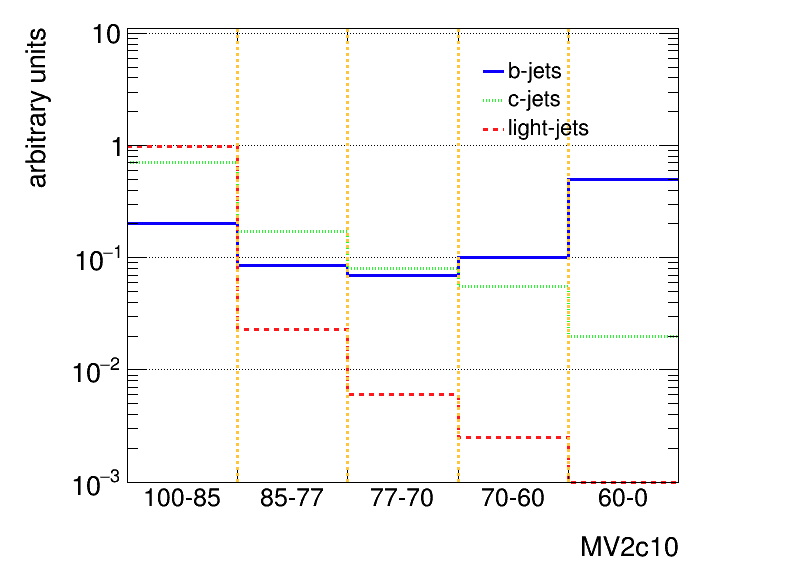
\includegraphics[width=0.7\textwidth]{PCBT}
  \caption[Shapes of the pseudo-continuous b-tagging quantiles for different jet
  flavours.]{Shapes of the PCBT quantiles for $b$-,$c$-, and light-jets.}
  \label{fig:PCBT_quant}
\end{figure}
Events that fall in the bins with ranges 70~--~60~\% and 60~--~0~\% have their
MV2c10 score stored for use in the analysis. Events in the other bins are not
tagged as $b$-jets.

\subsection{Truth Tagging}
\label{subsec:truth-tagging}

Removing all events that fail the cut associated with the 70~\% working point
results in loss of many events. This leaves us with a low number of events for
analysis, which is not ideal as many of the techniques used for categorising
events have performance conditional on the available number of events. Instead
of simply throwing these events away it is possible to keep all events that were
simulated to have a $b$-hadron decay and instead weight distributions by a
factor which represents the probability that an event would in fact be
$b$-tagged and enter into the final distribution. This procedure is known as
truth tagging, since the information as to whether a $b$-hadron is truly present
in a simulated event is utilised, this does not use any information relating to
the true nature of jets in the data as this is unknowable. In order to draw easy
comparisons, tagging directly with the MV2c10 algorithm is referred to as direct
tagging.

Given that our events contain more than one jet in all cases it is required to
develop a of way of generating truth tag weights for events based on all the
jets in the event. This weight is calculated as the product of the $b$-tagging
efficiency for each $b$-jet, multiplied by the complement of the $b$-tagging
efficiency for each non $b$-jet. In case the number of jets in a given event
($m$) exceeds the number of required tagged jets in the analysis ($n=2$) all
possible combinations of jets which satisfy the analysis selection are
considered.

The probability to choose specific combination of truth tagged jets can be
calculated as in appendix~\ref{app:truth-tag-probability}. A single truth tagged
combination can be selected based on this probability, and the event is then
scaled by the factor $w_{\mathrm {TT}}$. In practice due to differences between
the cumulative and pseudo-continuous $b$-tagging efficiency distributions a
modified version of truth tagging must be applied in the
analysis~\cite{VHObjectNote2019}.

\subsection{Hybrid Tagging}
\label{subsec:hybrid-tagging}
There exists disagreement between direct-tagged and truth-tagged events which
means that truth tagging cannot directly be applied to events in the analysis.
This is because direct tagging is the only strategy which can be used on data
and so we can only assume that direct-tagged distributions in simulation will
describe the shape and normalisation of distributions in the data. This problem
is solved by implementing so-called hybrid tagging. The hybrid tagging strategy
involves the following steps:
\begin{enumerate}
\item Divide the jets of each event in two groups, depending on the truth tag
  flavour: a group with only true $b$-jets and the other with non $b$-jets.
  
\item All $b$-jets in the first group are direct tagged.
  
\item  The remaining group of c- and light-jets is truth tagged imposing a
  number of tagged jets proportional to the difference between the number of
  required jets in the signal region and the number of true $b$-jets in the first
  group passing the b-tag requirement.
\end{enumerate}
Distributions of $t\bar{t}$ and $W+$jets are shown in
figures~\ref{fig:truth_tag_validation_tt}~and~\ref{fig:truth_tag_validation_wjets}.
Which show direct, truth and hybrid-tagged distributions. It can be seen that
the closure of hybrid-tagged events is much better than that of truth-tagged
events with respect to that of the direct-tagged events. Hybrid tagging is
therefore chosen as the analysis strategy.
\begin{figure}[ht]
  \centering
  \subfloat[]{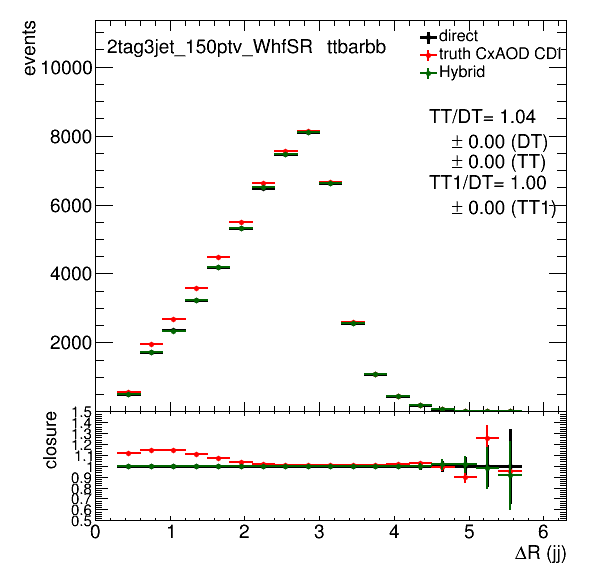
\includegraphics[width=0.48\textwidth]{TRF_2tag3jet_150ptv_WhfSR_ttbarbb_dRBB}}
  \subfloat[]{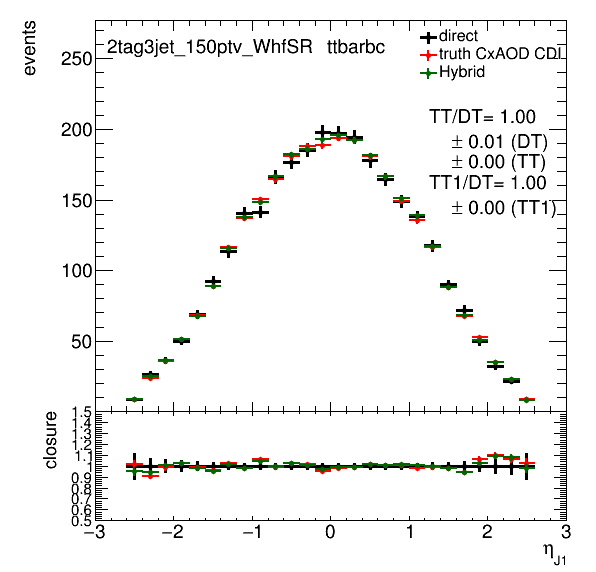
\includegraphics[width=0.48\textwidth]{TRF_2tag3jet_150ptv_WhfSR_ttbarbc_j1VecCorrEta}}
  \\
  \subfloat[]{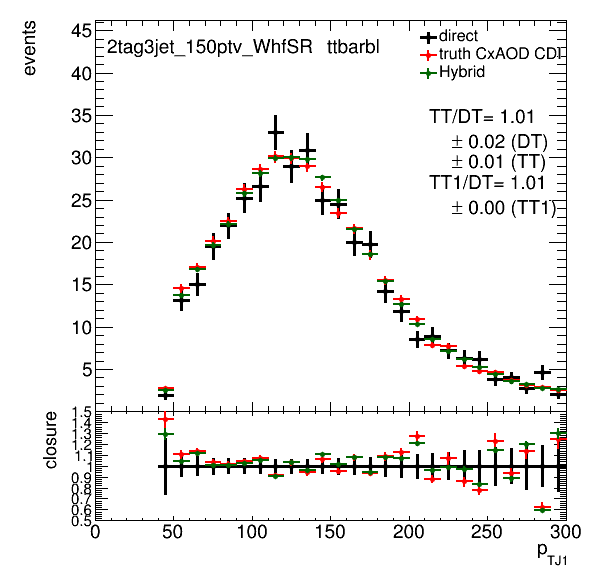
\includegraphics[width=0.48\textwidth]{TRF_2tag3jet_150ptv_WhfSR_ttbarbl_j1VecCorrPt}}
  \caption[A comparison of tagging strategies in $t\bar{t}$ events.]{Histograms of
    events using the direct tagging, truth tagging and hybrid tagging strategies
    are shown in black, red and green respectively. (a) $ \Delta R(\text{b, b})$
    distribution of $t\bar{t}$ events only including events with two $b$-jets. (b)
    $\eta$ distribution of $t\bar{t}$ events only including events with one
    $b$-jet and one $c$-jet. (c) $p_T$ distribution of the leading jet in
    $t\bar{t}$ events with one $b$-jet and one light-jet.}
  \label{fig:truth_tag_validation_tt}
\end{figure}
\begin{figure}[ht]
  \centering
  \subfloat[]{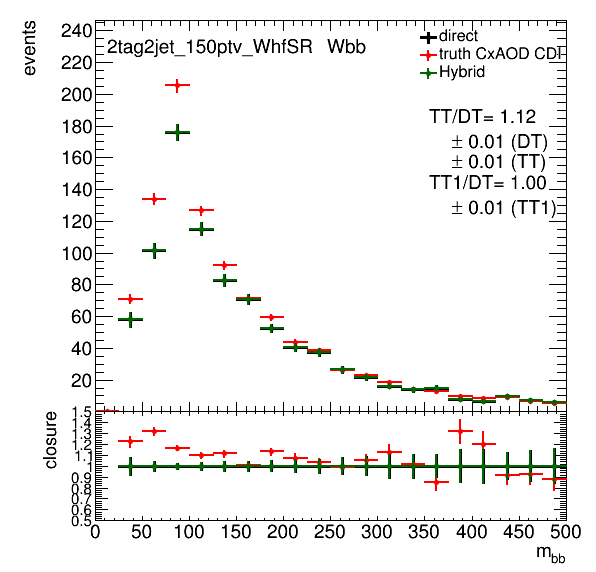
\includegraphics[width=0.48\textwidth]{TRF_2tag2jet_150ptv_WhfSR_Wbb_mBB}}
  \subfloat[]{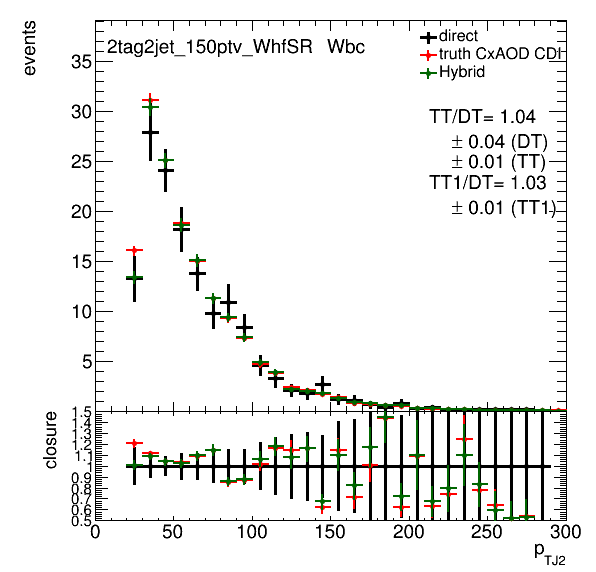
\includegraphics[width=0.48\textwidth]{TRF_2tag2jet_150ptv_WhfSR_Wbc_j2VecCorrPt}}
  \\
  \subfloat[]{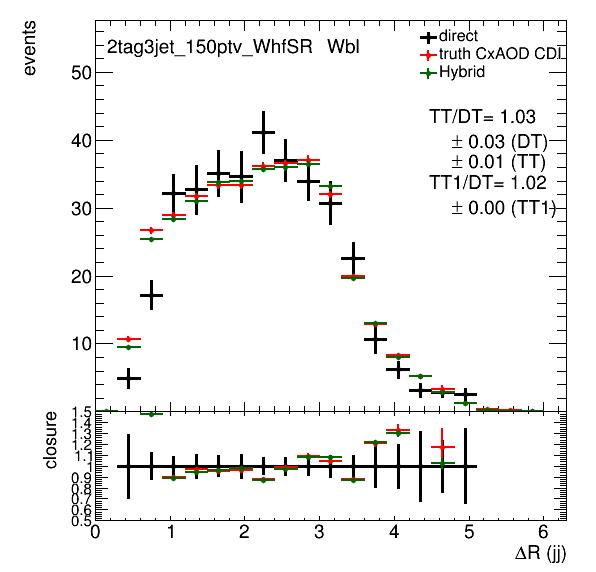
\includegraphics[width=0.48\textwidth]{TRF_2tag3jet_150ptv_WhfSR_Wbl_dRBB}}
  \caption[A comparison of tagging strategie in W + jets events.]{Histograms of
    events using the direct tagging, truth tagging and hybrid tagging strategies
    are shown in black, red and green respectively. (a) $m_{bb}$ distribution in
    $W + bb$ events. (b) $p_T$ of the sub-leading jet for $W + bc$ events. (c)
    $\Delta R(\text{jet, jet})$ distribution for $W + bl$.}
  \label{fig:truth_tag_validation_wjets}
\end{figure}

\clearpage
\newpage
\section{Missing Transverse Momentum}
\label{sec:met}
This section describes how $E_{\mathrm{T}}^{\text{miss}}$ is calculated. The calculation is based
on the assumption that partons entering into the hard scatter interaction have
zero transverse momentum when they collide. This is not true due them having
Fermi energy~\cite{fermi-energy}, but the transverse momentum induced by this
phenomenon is minimal and therefore is ignored. Given this assumption
$E_{\mathrm{T}}^{\text{miss}}$ is calculated as the negative vector sum of the $p_{\mathrm{T}}$ of
photons, electrons, muons, taus, and jets. There is also an additional soft term
that enters into the sum which is made up of all good quality tracks that aren't
associated with any of the aforementioned objects. These tracks must be
associated with the primary vertex and therefore are robust against pileup. A
second formulation of $E_{\mathrm{T}}^{\text{miss}}$ called $E_{T, Trk}^{\text{miss}}$ is
formulated just using inner detector tracks, it is even more robust to pileup
but cannot account for neutral particles which do no leave tracks in the inner
detector. One more variable known as $E_{\mathrm{T}}^{\text{miss}}$-significance is also
calculated as
\begin{equation}
  E_{\mathrm{T}}^{\text{miss}}\text{-significance} =
  \frac{E_{\mathrm{T}}^{\text{miss}}}{\sqrt{\Sigma p_{\mathrm{T}}^e + \Sigma p_{\mathrm{T}}^\mu + \Sigma p_{\mathrm{T}}^{jet}}},
  \label{eq:metsig}
\end{equation}
where the denominator is clearly proportional to the $E_{\mathrm{T}}^{\text{miss}}$
resolution and therefore making cuts on this variable simulates making harder
cuts on $E_{\mathrm{T}}^{\text{miss}}$ with better resolution and looser cuts on
$E_{\mathrm{T}}^{\text{miss}}$ with poorer resolution.

\section{Overlap Removal}
Given all of the reconstruction methods described so far for different physics
objects there has yet been any mention of what happens if overlapping detector
activity could be reconstructed into more than one physics object. The treatment
of overlap depends on which physics objects are involved. Below is summary of
how different pairs of overlapping objects which are relevant to the analysis
are handled, in the summary a combined muon is one which has been reconstructed
with the combined muon reconstruction algorithm, that is to say it has tracks in
the ID and energy deposits in the ECAL.\\
$\bullet$ \textbf{tau-electron:} If $\Delta R(\tau,e)<0.2$, the $\tau$ lepton is
removed.\\
%
$\bullet$ \textbf{tau-muon:} If $\Delta R(\tau,\mu)<0.2$, the $\tau$ lepton is
removed, unless the $\tau$ lepton has $p_{\mathrm{T}}>50$~\GeV\ and the muon is not a combined
muon, then the $\tau$ lepton is not removed.\\
%
$\bullet$ \textbf{electron-muon:} If a combined muon shares an ID track with an
electron, the electron is removed. If a calo-tagged muon shares an ID track with
an electron, the muon is removed.\\
%
$\bullet$ \textbf{electron-jet:} If $\Delta R(\text{jet},e)<0.2$ the jet is
removed. For any remaining jets, if $\Delta R(\text{jet},e)<0.4$, the
electron is removed.\\
%
$\bullet$ \textbf{muon-jet} If $\Delta R(\text{jet},\mu)<0.2$ or the muon ID
track is ghost associated~\cite{PERF-2012-02, ghost-ac-01, ghost-ac-02} to
the jet, then the jet is removed if the following also holds. The jet has less
than three associated tracks with $p_{\mathrm{T}} > 500$~\MeV\ or the $p_{\mathrm{T}}$ ratio of the muon
and jet is larger than 0.5 and the ratio of the muon $p_{\mathrm{T}}$ to the sum of $p_{\mathrm{T}}$
of tracks with $p_{\mathrm{T}} > 500$~\MeV\ associated to the jet is larger than 0.7. For
any remaining jets, if $\Delta R(\text{jet},\mu)<\min(0.4, 0.04 + 10\ \GeV /
p_{\mathrm{T}}^{\mu})$, the muon is removed from the jet.\\
%
$\bullet$ \textbf{tau-jet:} If $\Delta R(\tau,\text{jet})<0.2$, the jet is
removed.

\section{Final Selection}
\label{sec:selection}

The final analysis selection varies between channels. There are however some
common selections to all three channels as the Higgs candidate does not differ
between them. All events must have at least two signal jets. These signal jets
must be $b$-tagged, events with between 0 or 1 $b$-tags are considered for study
and are not used in the final analysis, events with $\ge3$ $b$-tags are rejected
entirely. The leading $b$-jet must have $p_{\mathrm{T}} > 45$~\GeV. A key variable in the
analysis, the di-jet mass, $m_{jj}$ is reconstructed from the two leading jets,
in the case where both jets are $b$-tagged $m_{bb} \equiv m_{jj}$ and represent
the mass of the Higgs candidate.

The reconstructed momentum of $b$-jets can be enhanced with better resolution
with respect to other jets. This is achieved with so-called muon-in-jet and
$p_{\mathrm{T}}$-reco corrections~\cite{VHObjectNote2019}. Corrections are applied after
events pass the full analysis selection, but before other stages of the
analysis. These corrections are not used in the calculation of any
$E_{\mathrm{T}}^{\text{miss}}$ related variables.

\subsection{0--Lepton Channel Selection}
\label{sec:0lep-selection}

The vector boson candidate in the 0--lepton channel is a $Z$ boson decaying to
two neutrinos. In order to select events for this candidate a large amount of
$E_{\mathrm{T}}^{\text{miss}}$ is required (> 150~\GeV) and there must be exactly 0
\VH-loose leptons in the event. Whilst events with lower $E_{\mathrm{T}}^{\text{miss}}$
may come from the physical process we desire to measure the $E_{\mathrm{T}}^{\text{miss}}$
trigger thresholds require setting the cut at it's value, the efficiency is
~90\% for events with $E_{\mathrm{T}}^{\text{miss}} = 150$~\GeV\ and efficiency plateaus at
$E_{\mathrm{T}}^{\text{miss}} \approx 180$~\GeV.

There exists a non-trivial dependence of the trigger efficiency on activity of
jets in detector. This arises due to the fact that the calculation of
$E_{\mathrm{T}}^{\text{miss}}$ is simply the total transverse energy of the event minus the
transverse energy of all objects in the event. These effects are hard to model
and so a requirement is put on
\begin{equation}
  S_{\mathrm{T}} = \sum_i p_{\mathrm{T}}^i, \text{for } i \text{ jets in the event,}
\end{equation}
such that it must be greater than 120 \GeV\ for events with two total jets, and
greater than 150 \GeV\ for events with three total jets.

Due to the lack of charged leptons in the $Z \rightarrow \nu\nu$ decay there is
nothing to trigger on to suppress multi-jet background processes arising from
QCD. This background is also enhanced due to limitations of the calorimeter
performance. A set of so-called anti-QCD cuts are applied to deal with this
multi-jet background, they are as follows:
\begin{itemize}
\item $\lvert \Delta \Phi ( E_{\mathrm{T}}^{\text{miss}} ,
  E_{t, trk}^{\text{miss}} ) \rvert <$ 90 $^\circ$
\item $\lvert \Delta \Phi ( j_1 , j_2 ) \rvert <$ 140 $^\circ$, where $j_1$ and
  $j_2$ are the leading and sub-leading jets respectively,
\item $\lvert \Delta \Phi ( E_{\mathrm{T}}^{\text{miss}} , h ) \rvert >$ 120 $^\circ$
\item $\text{min} ( \lvert \Delta \Phi ( E_{\mathrm{T}}^{\text{miss}} ,
  \text{pre-sel. jets}) \rvert ) >$ 20 $^\circ$ for  2 jets,
  $>$ 30 $^\circ$ for 3 jets.
\end{itemize}
Where $E_{t, trk}^{\text{miss}}$ is defined as the missing transverse momentum
calculated from the negative vector sum of the transverse momenta of tracks
reconstructed in the inner detector and identified as originating from the
primary vertex. These cuts reduce the multi-jet background to approximately 1\%
of the total background in this channel.

\subsection{1--Lepton Channel Selection}
\label{sec:1lep-selection}

The vector boson candidate in the 1--lepton channel is a W boson decaying to one
charged lepton and one neutrino. In order to select for events of this signature
exactly one \WH-signal lepton is required. At low $p_{\mathrm{T}}$ there is increased
contribution from multi-jet processes, therefore the extra requirements of
$p_{\mathrm{T}}^{W} > 150$ \GeV\ and $E_{\mathrm{T}}^{\text{miss}} > 30$ \GeV are applied to mitigate
this. The latter cut is only applied in the electron channel.  

\subsection{2--Lepton Channel Selection}
\label{sec:2lep-selection}

The vector boson candidate in the 2--lepton channel is a $Z$ boson decaying to
two charged leptons. Exactly two \VH-loose leptons of the same lepton flavour
are required, additionally one of the leptons must pass the \ZH-signal
requirements. For events with two muons, it is required that the muons are of
opposite charge. Electron reconstruction suffers from a higher rate of charge
misidentification and so this requirement is not applied to events with two
electrons. The di-lepton invariant mass is confined to be around the $Z$ boson
mass peak, events require $81 < m_{\ell\ell} < 101$ \GeV. These cuts reduce
multi-jet backgrounds to negligible levels.

The presence of two visible leptons in this channel allows for the enhancement
to $b$-jets momentum resolution to be further improved. By inspecting the $Z\!H\!
\to\! \ell\ell b\bar{b}$ decay (see figure~\ref{fig:feyn-vhbb}) it is clear that
the momentum of the Higgs and vector boson candidates ought to be balanced. The
momentum resolution of the two charged leptons forming the $Z$ boson candidate
is better than that of the $b$-jets (even after corrections). The $b$-tagged
jets momentum can therefore be corrected with a kinematic fit. The kinematic fit
improves resolution by 20-30\% compared with the muon-in-jet corrected
quantities. This correction is only applied to events with 2 or 3 total jets as
the presence of more jets results in smearing of the effect over those
additional jets.
\begin{table}[ht]
  \centering
  \begin{tabular}{l l} 
    \toprule
    \multicolumn{2}{l}{\textbf{Common Selections}}\\
    Jets & $\geq$  2 signal jets  \\
    $b$-jets &  2 $b$-tagged signal jets \\
    Leading $b$-tagged-jet $p_{\mathrm{T}}$\  & $>$ 45 \GeV \\
         &\\
    \multicolumn{2}{l}{\textbf{0 Lepton}} \\
    Trigger & lowest un-prescaled $E_{\mathrm{T}}^{\text{miss}}$ triggers \\
    Leptons & 0 \VH-loose lepton \\
    $E_{\mathrm{T}}^{\text{miss}}$ & $>$ 150~\GeV  \\
    
    $S_{\mathrm{T}}$ & $>$ 120 (2 jets), $>$150 \GeV (3 jets)  \\
    $\lvert \text{min} \Delta \phi (E_{\mathrm{T}}^{\text{miss}}, \text{jet}) \rvert$ & $> 20\ensuremath{^\circ}$ (2 jets) , $> 30\ensuremath{^\circ}$(3 jets) \\
    $\lvert \Delta\phi(E_{\mathrm{T}}^{\text{miss}}, h) \rvert$ & $> 120\ensuremath{^\circ}$ \\
    $\lvert \Delta\phi(j_1, j_2) \rvert$ & $< 140\ensuremath{^\circ}$ \\
    $\lvert \Delta\phi(E_{\mathrm{T}}^{\text{miss}}, E_{T, \text{trk}}^{\text{miss}}) \rvert$ & $< 90\ensuremath{^\circ}$ \\
    $p_{\mathrm{T}}^V$ regions & [150, 250]~\GeV, [250, $\infty$]~\GeV  \\
         &\\
    \multicolumn{2}{l}{\textbf{1 Lepton}} \\
    Trigger &  $e$ channel: un-prescaled single electron \\
         & Tables 6 and 7 of Ref.~\cite{VHobjectsupportnote}\\
         & $\mu$ channel: see 0--lepton triggers \\
    Leptons & 1 \WH-signal\ lepton \\
         &  $>1$~\VH-loose\ lepton veto \\
    $E_{\mathrm{T}}^{\text{miss}}$   & $>$ 30~\GeV ($e$ channel) \\
    $p_{\mathrm{T}}^{V}$ regions & [150, 250]~\GeV, [250, $\infty$]~\GeV  \\ 
         &\\
    \multicolumn{2}{l}{\textbf{2 Lepton}}\\
    Trigger &  un-prescaled single lepton\\
         & Tables 6 and 7 of Ref.~\cite{VHobjectsupportnote}\\
    Leptons & 2 \VH-loose\ leptons \\
         & ($\ge$ 1 \ZH-signal\ lepton) \\
         &  Same flavor, opposite-charge for $\mu\mu$ \\
    $m_{\ell\ell}$   & 81 $< m_{\ell\ell} <$ 101~\GeV \\
    $p_{\mathrm{T}}^{V}$ regions & [75,150], [150, 250], [250, $\infty$]~\GeV  \\
    \bottomrule
  \end{tabular}
  \caption[The analysis event selection.]{Summary of the signal event selection
    in the 0--, 1-- and 2--lepton analyses.}
  \label{tab:event-selection}
\end{table}